%\chapter{Character of Energy and Electron Transfer Illustrated Using Pairs
%         and Triples of Atoms}
\chapter{Geometric Influence on ICD and ETMD3  Illustrated Using Pairs and Triples of Atoms}
\label{chapter:geom}
Decomposing every system by pairs and triples of atoms is a very useful
first order approximation to both the investigation of energies and
decay widths of a larger system. Pairs and triples are combinations of
two and three atoms, respectively.
These atoms do not necessarily need to form bonds between each other or
even be close, but they are characterized according to fixed internal
coordinates. Each pair and triple can be described by its properties
which are in first order of approximation independent of further, eventually
present, atoms. In the following, this approach is going to be called
model of pairs and triples.

In case of the electronic decay processes one is interested in the
energies of the initial $E_{in}$ and the final states $E_{fin}$ of
the corresponding processes in order to determine, whether a channel $\beta$
is open, i.e., in accordance with energy conservation, or not. When the channel
is open, the excess energy is carried away by the emitted electron $E_{sec}$
in form of its kinetic energy. These energies can in the model
of pairs and triples be approximated to be

\begin{align}
 E_{in}^\beta  &= SIP(X_{in}^\beta) \label{equation:E_in}\\
 E_{fin}^\beta &= SIP(X_{fin1}^\beta) + SIP(X_{fin2}^\beta) + \frac 1d
           \label{equation:E_fin}\\
 E_{sec}^\beta &= E_{in}^\beta - E_{fin}^\beta \label{equation:E_sec}
\end{align}
where $X_{in}$ denotes the initially ionized atom and
$X_{fin1}$ and $X_{fin2}$ describe the two ionized
atoms in the final state. $\beta$ denotes the decay channel characterized
by the quantum numbers of the ionized atoms in the pairs
and triples and $d$ denotes the interatomic distance between the atoms
$X_{fin1}$ and $X_{fin2}$. The initially ionized atom $X_{in}$ can
coincide with one or both of
the final state atoms
$X_{fin1}$ and $X_{fin2}$. As explained in
chapter \ref{chapter:autoionization}, the distribution
of the vacancies over the different
atoms determines the kind of electronic decay process at hand. Hence, in an
Auger process all three atoms would coincide, for an ICD $X_{in}$
would coincide with one of $X_{fin1}$ and $X_{fin2}$ and for an \ac{ETMD}3
all ionized states are located on different atoms.

In all autoionization processes considered, a second electron
is emitted with the kinetic energy $E_{sec}$. If $E_{sec}<0$, then
the final state energy is higher than the initial state energy and the
process is energetically not accessible. Hence, the corresponding channel
is closed.

This ad hoc approach easily allows to correct for energetic shifts of
ionization potentials as observed in larger clusters.

The decay widths of the pairs and triples can be estimated with
different accuracy, but in general, the total decay width $\Gamma$ of
a system is the sum over the decay widths of all channels $\beta$ for
all possible pairs or triples $i$.

\begin{equation}
  \Gamma = \sum\limits_{i,\beta}\Gamma_{i,\beta}
\end{equation}


\section{Influence of the Geometry on ICD processes} \label{section:icd_geom}

\subsection{Geometry Dependence of the ICD Channel Openings and Closings}
In case of the \ac{ICD} process, the atoms $X_{in}$ and one of
the finally ionized atoms $X_{fin1}$ and $X_{fin2}$ coincide. For the sake of simplicity
it is now assumed that this atom is $X_{fin1}$. $d$ is then the interatomic distance
$R$ of $X_{fin1}$ and $X_{fin2}$.

\begin{figure}[h]
 \centering
 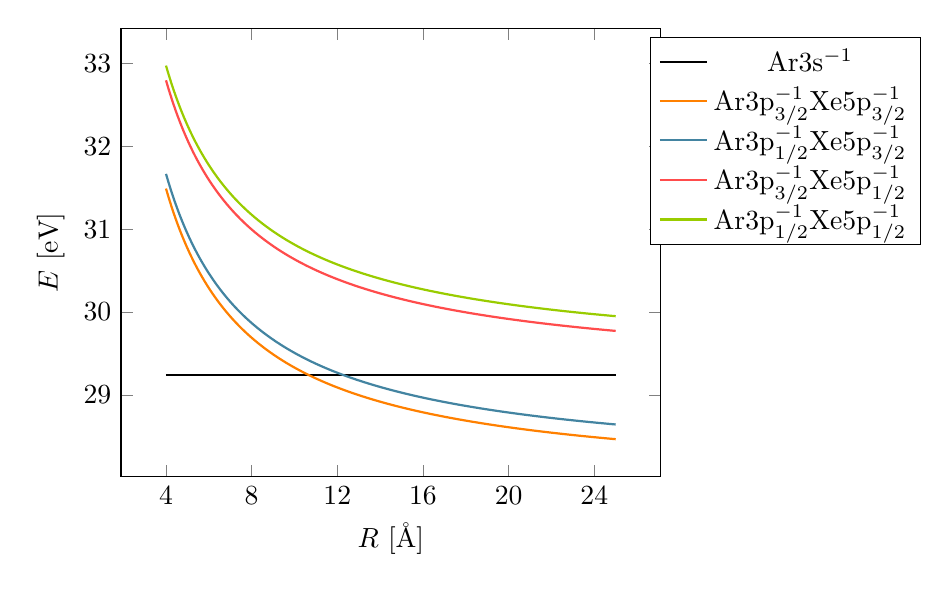
\begin{tikzpicture}
    \begin{axis}[domain=4.0:25,
                 samples = 200,
                 xtick={4.0,8.0,...,24},
                 %xticklabels={$-\pi$,$-\frac \pi 2$,0,$\frac \pi 2$,$\pi$},
                 cycle list name = exotic,
                 legend style={anchor= north west},
                 xlabel={$R$ [\AA]},
                 ylabel={$E$ [eV]}
                 ]
      \addplot+[
                mark = none,
                black,
                thick
               ]
               {29.239};
      \addlegendentry{Ar3s$^{-1}$};
      \addplot+[
                mark = none,
                thick
               ]
               {15.7596 + 12.1298 + 14.39964 / x};
      \addlegendentry{Ar3p$_{3/2}^{-1}$Xe5p$_{3/2}^{-1}$};
      \addplot+[
                mark = none,
                thick
               ]
               {15.9371 + 12.1298 + 14.39964 / x};
      \addlegendentry{Ar3p$_{1/2}^{-1}$Xe5p$_{3/2}^{-1}$};
      \addplot+[
                mark = none,
                thick
               ]
               {15.7596 + 13.4363 + 14.39964 / x};
      \addlegendentry{Ar3p$_{3/2}^{-1}$Xe5p$_{1/2}^{-1}$};
      \addplot+[
                mark = none,
                thick
               ]
               {15.9371 + 13.4363 + 14.39964 / x};
      \addlegendentry{Ar3p$_{1/2}^{-1}$Xe5p$_{1/2}^{-1}$};
      %\draw[] (axis cs:\pgfkeysvalueof{/pgfplots/xmin},29.239) -- (axis cs:\pgfkeysvalueof{/pgfplots/xmax},29.239);
    \end{axis}
\end{tikzpicture}

 \caption{Initial and final state energies of the ICD channels of ArXe in the
          model of pairs. Both the four relativistic channels and
          the non-relativistic estimate are shown. From the distance on, where
          the final state energy is lower than the initial state energy, the
          decay channel is open.}
 \label{figure:ArXe_energy_curves_unshifted}
\end{figure}

The ArXe dimer is chosen as an illustrative example in order to show the distance
dependency of the final state energies compared to the initial state
in the model of pairs using
ionization properties of the corresponding atoms given in Table
\ref{table:noble_atom_properties}.
In Figure \ref{figure:ArXe_energy_curves_unshifted} the energy of
the Ar3s$^{-1}$ initial
state is assumed to be constant, independent of any stabilization by the
neighbour and drawn as a black line. Additionally both the
curves of the four final states of the relativistic description and
a hypothetical non-relativistic curve calculated by the means of
equation (\ref{equation:E_fin}) are shown.

For small distances up to \unit[10]{\AA}, all channels are closed. As soon as the final
state curves cross the energy of the initial state
the respective channels open. For the four relativistic channels these
channel opening distances are
\unit[10.67]{\AA}, \unit[12.29]{\AA} and \unit[334.1]{\AA}
for the Ar3p$_{3/2}^{-1}$Xe5p$_{3/2}^{-1}$,
Ar3p$_{1/2}^{-1}$Xe5p$_{3/2}^{-1}$ and Ar3p$_{3/2}^{-1}$Xe5p$_{1/2}^{-1}$
channels, respectively.
The sum of the two ionization potentials of the
Ar3p$_{1/2}^{-1}$Xe5p$_{1/2}^{-1}$ channel are already higher than
the initial state energy. Therefore this channel never opens.
In the non-relativistic treatment, the atomic ionization energies of the
Ar3p and the Xe5p are estimated by the statistically weighted average of the
p$_{3/2}$ and the p$_{1/2}$ ionization energies. The non-relativistic
opening distance would then be
\unit[16.84]{\AA}.

Considering a distinct distance
in an experiment as many secondary electron peaks would be observed as
energetically distinguishable channels are open. The non-relativistic
treatment predicts one single peak, whereas the relativistic approach takes
care of the different channels due to spin-orbit coupling and therefore is
able to predict the correct number of peaks for a reasonable choice of initial
and final state energies.

Hence, for an ArXe dimer with an equilibrium distance of \unit[4.04]{\AA}
all ICD channels are closed. As can be seen in the discussion of mixed
ArXe clusters, that in case of shifted curves, ICD channels might
open at atomic distances, where the decay widths are non-negligible.


\subsection{Geometry Dependence of the ICD Decay Widths}

The decay widths $\Gamma$ in the asymptotic description of equation
(\ref{reltheolifetime_exp}) shows a pure $R^{-6}$ behaviour.
However, this does not contain any information about whether the channel is
open and hence, whether such a process would be observable. Therefore,
in Figure \ref{figure:ArXe_gamma_unshifted} the decay width is plotted
over $R$ with the additional condition, that the corresponding channel needs
to be open at the distance of interest for both the relativistic treatment
and the non-relativistic analogon.

\begin{figure}[h]
  \centering
  \begin{tikzpicture}[scale=1.0]

\begin{loglogaxis}[%scale=1.5,
             domain=3:30,
             y domain=1E-8:10,
             restrict expr to domain={y}{1E-8:15},
             xlabel={R in \AA},
             xtick={2,4,...,10,12,15,...,25},
             xticklabels={2,4,6,8,10,12,15,20,25},
             ylabel={$\Gamma(R)$ in \unit{eV}},
             %title={Parameter Fitting of NeNe and NeAr Decay Widths}
             ]

\addplot[%only marks,
         mark=x,
         thick,
         diplom1
        ]
        table[
        x expr = \thisrowno{0},
        y expr = \thisrowno{1}
        ]
        {data/arxe_nrel_unshifted.dat};
        \addlegendentry{nrel unshifted};
	
	
\addplot[%only marks,
         mark=x,
         thick,
         diplom2
        ]
        table[
        x expr = \thisrowno{0},
        y expr = \thisrowno{1}
        ]
        {data/arxe_rel_unshifted.dat};
        \addlegendentry{rel unshifted};
	
\end{loglogaxis}
\end{tikzpicture}


  \caption{Decay widths of the ArXe dimer in relativistic and non-relativistic
           treatment plotted over the interatomic
           distance $R$. The initial and final state energies were determined
           from unshifted experimental atomic ionization potentials. Only such
           channels are considered, which are open at the corresponding
           distances.}
  \label{figure:ArXe_gamma_unshifted}
\end{figure}

In this double logarithmic plot, the decay width determined non-relativistically
is a straight line starting
from the opening distance of \unit[16.84]{\AA}.
In contrast to this, the relativistic treatment shows a decay at much smaller
distances, as was to be expected from the smaller opening distance of the
Ar3p$_{3/2}^{-1}$Xe5p$_{3/2}^{-1}$ channel. Already from this point it
can be seen, that the non-relativistic treatment is not sufficient for systems
with a large spin-orbit coupling. Between \unit[12]{\AA} and
\unit[13]{\AA} the relativistic decay width s approximately constant rather than
decreasing with $R^{-6}$.
In this region, the second channel, Ar3p$_{1/2}^{-1}$Xe5p$_{3/2}^{-1}$, opens
and its contribution to the decay is added to the decay width of the first
decay channel. However, at distances where the non-relativistic channel is open,
for the distances shown in this illustration, the non-relativistic decay width
is higher than the total relativistic one. This observation stems from the fact,
that in a first order approximation, when all channels are open in the relativistic
treatment, the sum over their decay widths has to equal the non-relativistic one.
In the case of the ArXe dimer and the distances shown in Figure
\ref{figure:ArXe_gamma_unshifted}, not all relativistic channels are open, and
hence the non-relativistic treatment overestimates the decay width.

The sum over the relativistic decay widths will for these calculations never
exactly give the non-relativistic result, because even though a thorough
partitioning of the lifetime $\tau$ and the ionization cross section
$\sigma(\omega_{vp})$ are taken care of, the cross section as well as the decay
width depend on the energy of the virtual photon $\omega_{vp}$ non-linearly and this
energy differs for different ionization energies of the final state of the
initially ionized atom.
